
% The \phantomsection command is needed to create a link to a place in the document that is not a
% figure, equation, table, section, subsection, chapter, etc.
% https://tex.stackexchange.com/questions/44088/when-do-i-need-to-invoke-phantomsection
\phantomsection

% Multiple-language document - babel - selectlanguage vs begin/end{otherlanguage}
% https://tex.stackexchange.com/questions/36526/multiple-language-document-babel-selectlanguage-vs-begin-endotherlanguage
\begin{otherlanguage*}{brazil}

\chapter{Desenvolvimento}

Nesta seção, será abordada a LTI do Beecrowd, que simplifica a integração entre o Moodle e a plataforma Beecrowd. Serão apresentados também os detalhes da implementação da aplicação web do sistema especialista, desenvolvida para auxiliar professores e alunos no esclarecimento de dúvidas recorrentes sobre as questões do Beecrowd, facilitando a adaptação de ambos ao uso da plataforma.

\section{LTI BEECROWD}

Com a disponibilização de uma ferramenta LTI pelo Beecrowd, visando facilitar sua integração com o Moodle, foi elaborado um manual detalhado para orientar o administrador do Moodle na configuração dessa LTI (Apêndice A).

Para configurar uma LTI externa, o administrador deve acessar "Administração do site", selecionar "Plugins" e, em "Módulos de atividade", escolher "Ferramenta externa" e clicar em "Gerenciar ferramentas". Em seguida, deve clicar em "Configurar uma ferramenta manualmente" e preencher os campos conforme as instruções especificadas no Manual de Configuração da LTI Beecrowd no Moodle (Apêndice A). Após a configuração, será possível visualizar os detalhes da ferramenta, os quais deverão ser enviados ao Beecrowd para estabelecer a comunicação entre as plataformas.

Além disso, foi desenvolvido um manual de uso da LTI Beecrowd (Apêndice B), direcionado aos professores que desejam utilizar o Beecrowd como suporte educacional em sala de aula. Esse manual instrui os docentes sobre como criar uma atividade do Beecrowd no Moodle, orientar o acesso dos estudantes e transferir as notas obtidas no Beecrowd para o Moodle.

Após seguir o guia do Manual de Uso da LTI Beecrowd (Apêndice B), duas atividades ficam disponíveis na página do curso, apresentadas como "botões" visuais. A primeira atividade, que é ocultada para os estudantes (Imagem 23), permite ao professor acessar o Beecrowd Academic (Imagem 24) para configurar disciplinas, criar listas de exercícios para os alunos e enviar as notas para o Moodle.

\begin{figure}[H]
    \centering
            \caption{Atividade para o professor acessar o Beecrowd Academic}
            \label{fig:ModeloConceitual}
        
\includegraphics[scale=0.35]{pictures/apendices/apendice_b_5.png}
        \fonte{Produzido pela autora.}
\end{figure}

\begin{figure}[H]
    \centering
            \caption{Beecrowd Academic}
            \label{fig:ModeloConceitual}
        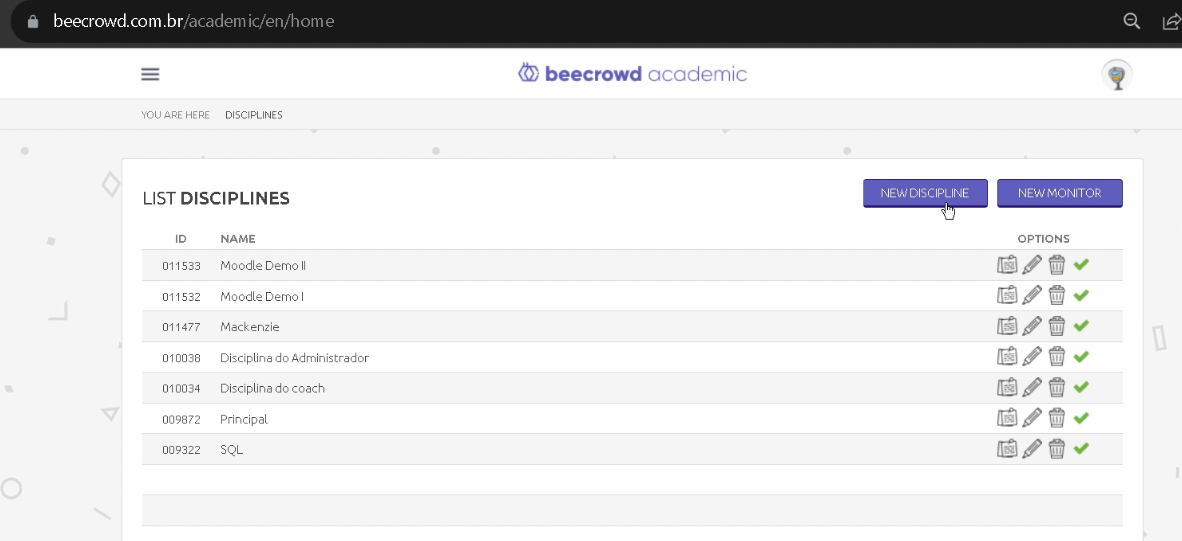
\includegraphics[scale=0.38]{pictures/desenvolvimento/lti_beecrowd_academic.png}
        \fonte{Produzido pela autora.}
\end{figure}

A segunda atividade, acessível aos estudantes (Imagem 25), redireciona-os diretamente para a página no Beecrowd da lista de exercícios criada pelo professor (Imagem 26), sem necessidade de cadastro ou login. Assim, os estudantes podem resolver as atividades diretamente a partir dessa página. Esse botão também permite ao professor acessar a lista de exercícios criada, podendo verificar o progresso dos alunos, as tentativas realizadas e, quando desejado, enviar as notas para o Moodle.

\begin{figure}[H]
    \centering
            \caption{Atividade para o aluno acessar o Beecrowd}
            \label{fig:ModeloConceitual}
        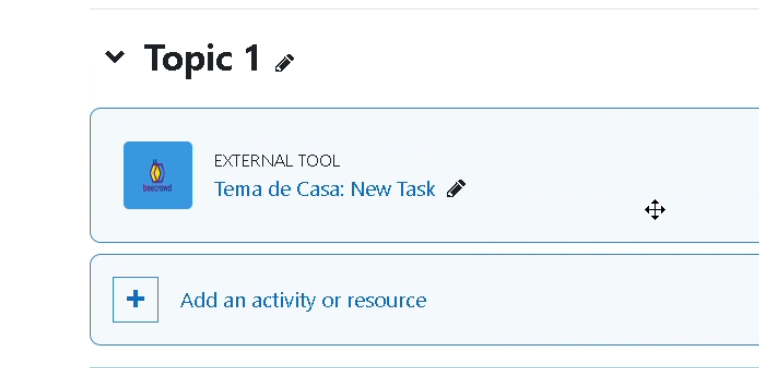
\includegraphics[scale=0.4]{pictures/desenvolvimento/lti_tarefa.png}
        \fonte{Produzido pela autora.}
\end{figure}

\begin{figure}[H]
    \centering
            \caption{Beecrowd do aluno}
            \label{fig:ModeloConceitual}
        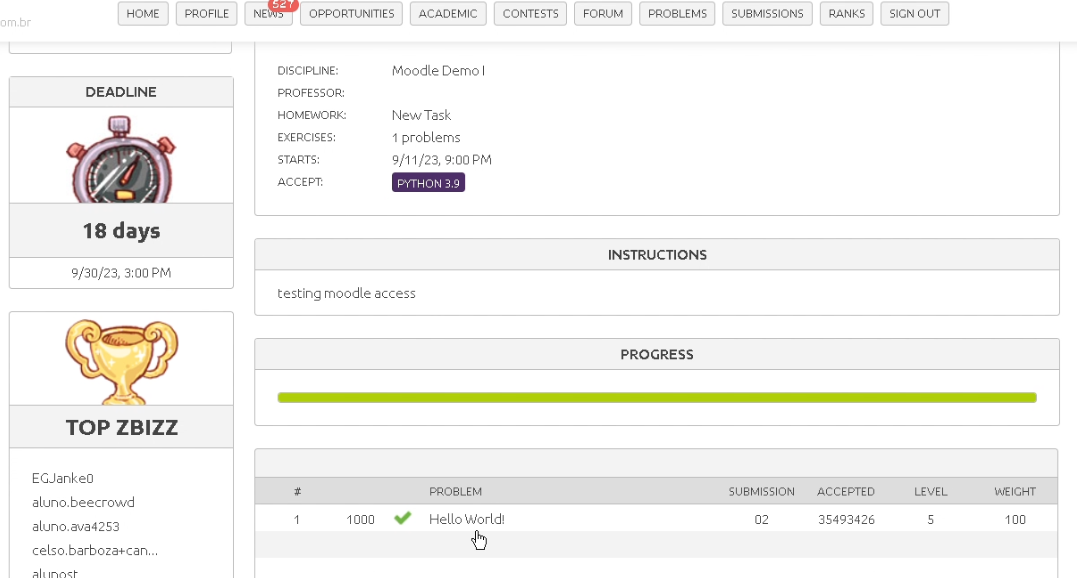
\includegraphics[scale=0.4]{pictures/desenvolvimento/lti_beecrowd_aluno.png}
        \fonte{Produzido pela autora.}
\end{figure}

\section{ARQUITETURA DE SOFTWARE}

A representação da integração é esquematizada na Figura 21, onde o plugin criado estabelece comunicação exclusivamente com a LTI do Beecrowd. A LTI (Learning Tools Interoperability) do Beecrowd, funcionando como uma interface receptora de requisições, interage diretamente com o site do Beecrowd, retornando dados ao plugin. Com essa abordagem, a integração permite que, ao ter o plugin incorporado ao Moodle, professores e alunos possam acessar e utilizar os recursos do Beecrowd pelo Moodle.

\begin{figure}[h!]
    \centering
            \caption{Arquitetura da Integração Moodle-Beecrowd}
            \label{fig:ModeloConceitual}
        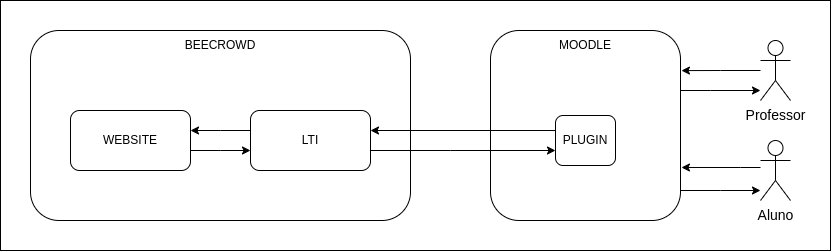
\includegraphics[scale=0.5]{pictures/arquitetura.png}
        \fonte{Produzido pela autora.}
\end{figure}

Já a figura 22 mostra o diagrama de caso de uso do plugin desenvolvido para integrar o Moodle ao Beecrowd. O diagrama de caso de uso é uma representação visual crucial para compreender e planejar a interação entre os usuários e um sistema, esboçando de forma clara e sistemática as diversas funcionalidades que professores e alunos podem realizar, evidenciando as interações entre eles e o sistema integrado. Cada "caso de uso" no diagrama encapsula uma atividade específica, delineando como os usuários interagem com o sistema para atingir seus objetivos. Essa representação gráfica oferece uma visão abrangente e estruturada das diferentes operações disponíveis, estabelecendo uma base sólida para o desenvolvimento, implementação e compreensão do sistema integrado Moodle-Beecrowd.

\begin{figure}[h!]
    \centering
            \caption{Diagrama de Caso do Plugin da Integração Moodle-Beecrowd}
            \label{fig:ModeloConceitual}
        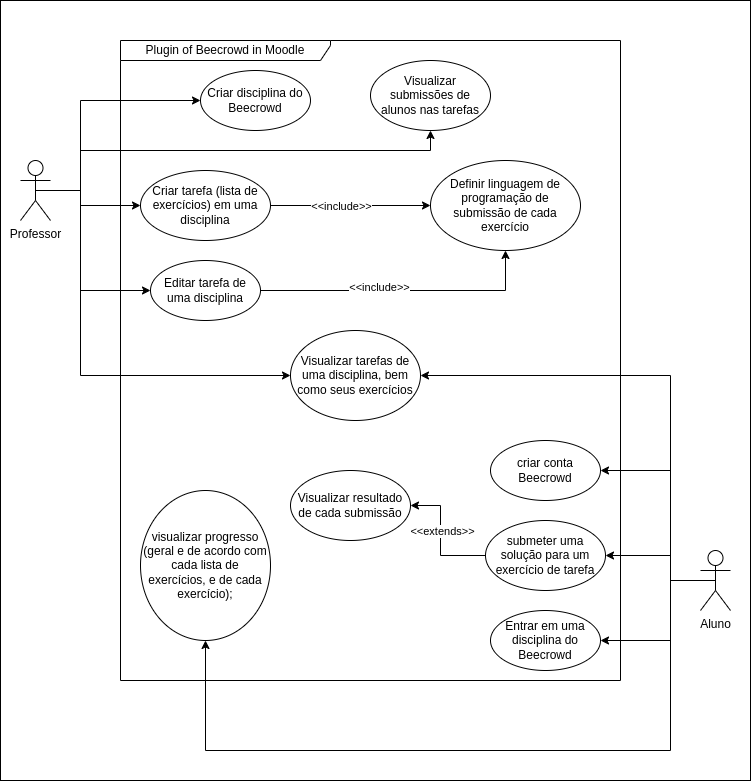
\includegraphics[scale=0.6]{pictures/caso_de_uso.png}
        \fonte{Produzido pela autora.}
\end{figure}

Assim, o professor pode, ao usar o plugin no Moodle, criar disciplinas do Beecrowd, criar tarefas, ou seja, lista de exercícios, em uma disciplina do Beecrowd, editar tarefas de uma disciplina, definir a linguagem de programação de submissão de cada exercício em uma tarefa, visualizar tarefas de uma disciplina, bem como seus exercícios, e, por fim, visualizar as submissões de alunos nas tarefas. 

Já o aluno pode criar uma conta do Beecrowd pelo Moodle, ao usar a funcionalidade adicionada pelo plugin em uma disciplina, e entrar em uma disciplina do Beecrowd criada pelo seu professor, e disponibilizada no Moodle pelo seu professor. Também pode submeter soluções para exercícios de tarefas criadas pelo seu professor, e, assim, pode visualizar o resultado de suas submissões realizadas. Aleḿ disso, consegue visualizar seu progresso geral da disciplina, ou de cada tarefa disponibilizada no Moodle através do plugin.

\section{REQUISITOS DA APLICAÇÃO}

\subsection{Regras de Negócio}

\textbf{RG1 – Importação de Notas:} O sistema deve importar as notas do Beecrowd para o Moodle apenas para disciplinas e tarefas previamente associadas, evitando importações não autorizadas;

\vspace{12pt}

\textbf{RG2 – Cadastro Automático de Alunos:} Alunos podem se cadastrar automaticamente no Beecrowd pelo Moodle somente se estiverem matriculados nas disciplinas habilitadas para uso do Beecrowd;

\vspace{12pt}

\textbf{RG3 – Criação Automática de Disciplina:} A criação automática de disciplinas no Beecrowd ao habilitar o uso deve seguir uma estrutura de nomenclatura padronizada para facilitar a identificação;

\vspace{12pt}

\textbf{RG4 – Visualização de Submissões:} A visualização de submissões de alunos no Beecrowd pelo Moodle só é permitida para professores associados às disciplinas correspondentes;

\vspace{12pt}

\textbf{RG5 – Submissão de Solução:} Alunos só podem submeter soluções no Beecrowd via Moodle para as listas de exercícios ativas e dentro dos prazos estabelecidos;

\vspace{12pt}

\textbf{RG5 – Acesso às Listas de Exercícios:} O acesso às listas de exercícios e questões no Moodle está disponível apenas durante o período em que a disciplina está em andamento.

\vspace{12pt}

\subsection{Requisitos Não Funcionais}

\textbf{RNF01 – Linguagem de Programação e Tecnologias Front-end:} O plugin deve ser desenvolvido utilizando a linguagem de programação PHP para a lógica de back-end e HTML, CSS e Javascript para adaptar o frontend;

\vspace{12pt}

\textbf{RNF02 – Interface Responsiva:} A interface do usuário deve ser responsiva e seguir as melhores práticas de design para garantir uma experiência do usuário consistente;

\vspace{12pt}

\textbf{RNF03 – Estrutura de Diretórios e Arquivos:} O código do plugin deve seguir a estrutura de diretórios e arquivos especificada na seção "Fundamentos Teóricos", na subseção "Plugin do Moodle";

\vspace{12pt}

\textbf{RNF04 – Padrões de Desenvolvimento:} O código do plugin deve aderir aos padrões de codificação estabelecidos para o desenvolvimento de plugins no ambiente Moodle, incluindo boas práticas de programação, documentação e modularidade para assegurar a qualidade e manutenibilidade do código;

\vspace{12pt}

\textbf{RNF05 – Diagrama UML:} A implementação do plugin deve seguir as especificações detalhadas no diagrama UML fornecido, garantindo que a estrutura e os relacionamentos definidos sejam fielmente reproduzidos no sistema;

\vspace{12pt}

\textbf{RNF06 – Integração com LTI (Learning Tools Interoperability):} O plugin deve ser desenvolvido com integração compatível com o padrão LTI, assegurando interoperabilidade eficaz com outras ferramentas educacionais que suportem esse padrão;

\vspace{12pt}

\textbf{RNF07 – Documentação do Plugin:} Deve ser fornecida uma documentação completa e clara, incluindo README, CHANGES e outros arquivos necessários, facilitando a instalação, configuração e utilização do plugin por parte dos administradores e usuários;

\vspace{12pt}

\textbf{RNF08 – Compatibilidade com Versões do Moodle:} O plugin deve ser compatível com as versões específicas do Moodle, conforme indicado nas diretrizes de suporte e requisitos do sistema, para garantir a funcionalidade em ambientes Moodle diversos;

\vspace{12pt}

\textbf{RNF09 – Segurança:} O plugin deve incorporar medidas de segurança adequadas para proteger contra vulnerabilidades conhecidas;

\vspace{12pt}

\textbf{RNF10 – Desempenho:} O plugin deve ser otimizado para garantir desempenho eficiente, minimizando tempo de carregamento e consumo de recursos do sistema, proporcionando uma experiência rápida e responsiva;

\vspace{12pt}

\textbf{RNF11 – Compatibilidade:} O plugin deve ser compatível com os principais navegadores (Chrome, Firefox, Safari) e dispositivos (desktop, tablet, mobile) para garantir uma experiência consistente.

\subsection{Requisitos Funcionais}

\textbf{RF01 – Importação de Notas do Beecrowd para o Moodle:} O sistema deve permitir a importação automática das notas dos alunos no Beecrowd para o Moodle;

\vspace{12pt}

\textbf{RF02 – Cadastro Automático no Beecrowd via Moodle:} Os alunos devem ter a opção de realizar o cadastro automaticamente no Beecrowd por meio do Moodle;

\vspace{12pt}

\textbf{RF03 – Criação Automática de Disciplina no Beecrowd:} Ao habilitar o uso do Beecrowd no Moodle para uma disciplina, o sistema deve criar automaticamente a correspondente disciplina no Beecrowd;

\vspace{12pt}

\textbf{RF04 – Visualização de Submissões no Beecrowd pelo Moodle:} Os professores devem ser capazes de visualizar as submissões dos alunos no Beecrowd, juntamente com os feedbacks fornecidos pelo Beecrowd, diretamente no Moodle;

\vspace{12pt}

\textbf{RF05 – Criação de Listas e Competições no Beecrowd pelo Moodle:} Professores devem poder criar listas de exercícios e competições no Beecrowd diretamente através do ambiente Moodle;

\vspace{12pt}

\textbf{RF06 – Submissão de Solução no Beecrowd via Moodle:} Alunos devem ser capazes de submeter suas soluções para as listas de exercícios do Beecrowd diretamente através do Moodle;

\vspace{12pt}

\textbf{RF07 – Acompanhamento do Progresso no Beecrowd pelo Moodle:} Professores devem conseguir visualizar o progresso de cada aluno, tanto de forma geral na disciplina quanto em relação a cada lista de exercícios, no Beecrowd, pelo Moodle;

\vspace{12pt}

\textbf{RF08 – Acompanhamento do Próprio Progresso pelo Aluno:} Alunos devem poder visualizar seu próprio progresso geral na disciplina, assim como o desempenho em cada lista de exercícios e em cada exercício específico, no Beecrowd, pelo Moodle;

\vspace{12pt}

\textbf{RF09 – Acesso às Listas de Exercícios e Questões no Moodle:} Alunos e professores devem conseguir abrir as listas de exercícios do Beecrowd, incluindo o acesso aos enunciados das questões, diretamente no Moodle;

\vspace{12pt}

\textbf{RF10 – Definição de Linguagem de Programação no Moodle:} Professores devem poder definir a linguagem de programação para submissão das questões no Beecrowd, diretamente no Moodle, a fim de minimizar erros na seleção de versões inadequadas do Python;

\vspace{12pt}

\textbf{RF11 – Visualização do Feedback de cada submissão de exercício do Beecrowd pelo Moodle:} Deve ser possível ao aluno visualizar o feedback do Beecrowd para cada submissão de exercício diretamente pelo Moodle.

\end{otherlanguage*}

